\chapter{3	Basics Intelligent Robotics}


\section{Basics}

\subsection{Machine Learning Basics}
\subsubsection{Agent \& Policy:}

An agent is an entity that learns to perform a specific behavior through interaction with its environment. In the context of this work, the agent corresponds to the robot, which has to execute a given action or task. The policy can be interpreted as the brain of the agent, determining which action to take next in a given situation in order to achieve the task objective. In our example, the policy controls the robot's motion and actions.  

Formally, a policy can be represented as  
\begin{align}
	\pi_\theta(a \mid s)  
\end{align}
which defines a probability distribution over actions $a$, conditioned on the current state $s$. In other words, the policy specifies how likely the agent is to select a particular action given its current observation of the environment.  

In the classical meaning, the action $a$ corresponds for example to a robot command, such as moving the gripper to a target position $(x, y, z)$ or setting a joint angle to a specific value with a defined velocity. The state $s$ represents the agent’s observation, which may include, for example, a sequence of recent camera images (e.g., the last four frames) as well as additional sensor inputs such as proprioceptive signals.

\subsubsection{Robot Trajectory:}

A robot trajectory describes how the robot moves from a starting state to a target state, including position, orientation and, if applicable, speeds, accelerations, and forces acting on the robot. A robot tracetory is a temporal sequence of actions and the resulting robot states.


\subsubsection{Annotation:}

Annotation refers to the process of labeling data. Data is provided with additional information. For example, class affiliations can be determined, target objects can be marked in images, or states and actions can be marked in robot trajectories. Annotated data, or labeled data, form the basis for supervised learning approaches.

Annotating refers to the process of labeling data, in which data is enriched with additional information. For example, this may include assigning class labels, marking target objects in images, or labeling states and actions within robot trajectories. Annotated, or labeled, data forms the foundation for supervised learning approaches.


\subsection{Core Machine Learning Categories}
There are various approaches to training an AI model for a robot. These involve methods from the four core machine learning categories, which can also be combined with one another:

\subsubsection{Supervised Learning: }

In supervised learning, a model is trained using labeled training data. This means that, for the input data, the output data to be predicted are known. The goal is to train a model that correctly predicts the output data and makes reliable predictions on unseen data. 


\subsubsection{Unsupervised Learning: }
In contrast to supervised learning, unsupervised learning uses unlabeled data for model training. The model tries to recognize structures, patterns or relationships in the data on its own. 

\subsubsection{Semi Supervised Learning: }
Semi-supervised learning is a combination of supervised and unsupervised learning. In this approach, a model is trained using a small amount of labeled data and a large amount of unlabeled data. The goal is to leverage the advantages of both approaches, particularly when annotating data is time-consuming or costl-intensive. This is relevant in robotics, as the data used in that field is often difficult to label.

\subsubsection{Reinforcement Learning: }

Reinforcement learning (RL) differs fundamentally from the previously mentioned approaches. Instead of learning from fixed datasets, an agent actively interacts with its environment. Through its actions, it influences the state of the environment and subsequently receives feedback in the form of rewards or penalties. 
The objective is to learn a strategy (= policy) that maximizes the cumulative reward over time for the given task.

The agent proceeds in its environment according to the trial-and-error principle to learn an optimal policy. Safety is a critical concern during training, as the agent may execute unpredictable actions while exploring the state space. For this reason, simulation environments are a central component of training and are frequently used for pre-training the policy. The policy is then subsequently fine-tuned in the real-world environment.














\section{Intelligent robots with Deep Learning}
In general, modern robot training distinguishes between two main approaches: imitation learning and reinforcement learning. Each approach uses a different strategy for training the robot model.
\begin{figure}
	\centering
	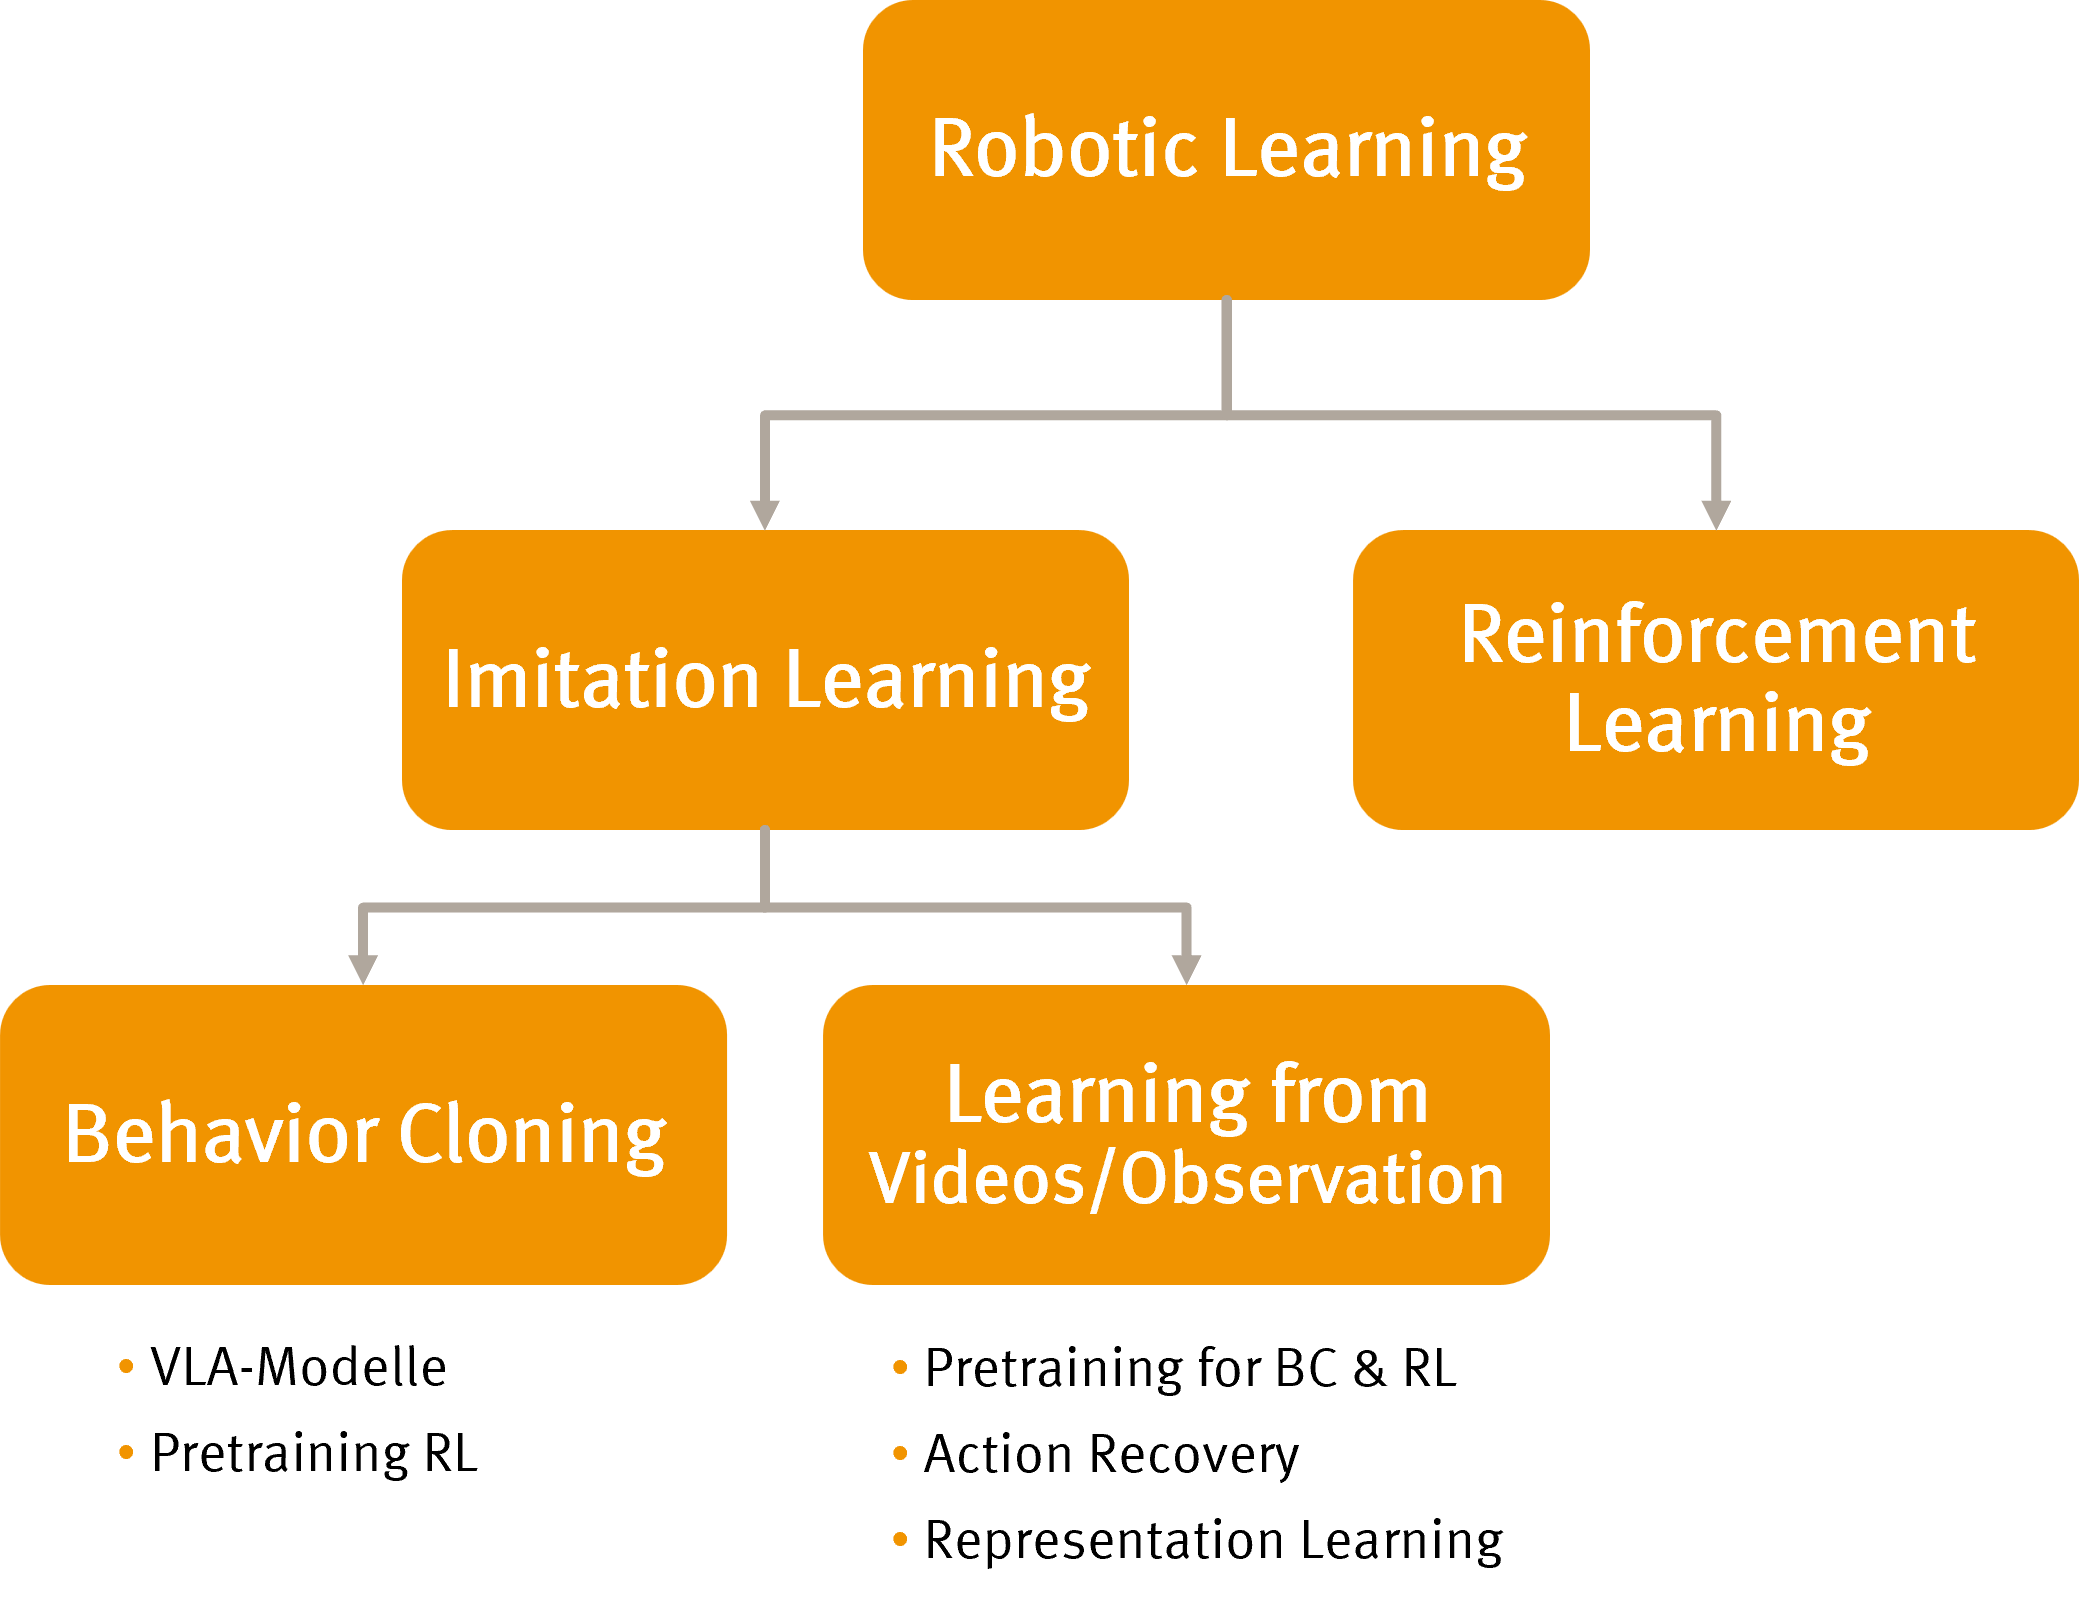
\includegraphics[width=0.6\linewidth]{./kapitel3_media/OverviewRoboticLearning.png}
	\caption[Overview Robotic Learning]{Overview Robotic Learning}
	\label{fig:overviewroboticlearning}
\end{figure}



\subsection{Reinforcement Learning}
Reinforcement learning is both a fundamental discipline of machine learning and a distinct approach within Robot Learning.
The agent learns a policy through trial and error using rewards. The actions performed by the agent are evaluated with a score, and this score is then used to gradually optimize the policy.

\subsection{Imitation Learning}
Imitation Learning or Learning from Demonstration is a general term for methods in which the agent derives or learns its behavior from expert demonstrations.

Imitation learning makes it possible to use "in the wild" videos—such as those found in great variety on the internet, for example on platforms like YouTube — to train AI models.

The demonstration videos can show a robot, a human, or even a loose sequence of actions, both in the real world or in a simulation environment, performing a specific task. However, videos without a clearly defined objective or with unknown activity can also be used.

This allows models to be trained to capture the visual and semantic relationships, as well as the physical dynamics of the real world. This, in turn, is a key prerequisite for the development of a generalist policy.
Imitation learning can be divided into Behavior Cloning and Learning from Videos/Observation.

\subsubsection{Behavior Cloning (BC)}

\begin{align}
	\sin(x+2\pi) &= \sin(x)\\
	\cos(x+2\pi) &= \cos(x)\\
	\cos(x) &= \sin\left(x+\frac{\pi}{2}\right)
\end{align}

